\documentclass[11pt,a4paper]{report}
\usepackage[textwidth=37em,vmargin=30mm]{geometry}
\usepackage{calc,xunicode,amsmath,amssymb,paralist,enumitem,tabu,booktabs,datetime2,xeCJK,xeCJKfntef,listings}
\usepackage{tocloft,fancyhdr,tcolorbox,xcolor,graphicx,eso-pic,xltxtra,xelatexemoji}

\newcommand{\envyear}[0]{2025}
\newcommand{\envdatestr}[0]{2025-04-08}
\newcommand{\envfinaldir}[0]{webdb/2025/20250408/final}

\usepackage[hidelinks]{hyperref}
\hypersetup{
    colorlinks=false,
    pdfpagemode=FullScreen,
    pdftitle={Web Digest - \envdatestr}
}

\setlength{\cftbeforechapskip}{10pt}
\renewcommand{\cftchapfont}{\rmfamily\bfseries\large\raggedright}
\setlength{\cftbeforesecskip}{2pt}
\renewcommand{\cftsecfont}{\sffamily\small\raggedright}

\setdefaultleftmargin{2em}{2em}{1em}{1em}{1em}{1em}

\usepackage{xeCJK,xeCJKfntef}
\xeCJKsetup{PunctStyle=plain,RubberPunctSkip=false,CJKglue=\strut\hskip 0pt plus 0.1em minus 0.05em,CJKecglue=\strut\hskip 0.22em plus 0.2em}
\XeTeXlinebreaklocale "zh"
\XeTeXlinebreakskip = 0pt


\setmainfont{Brygada 1918}
\setromanfont{Brygada 1918}
\setsansfont{IBM Plex Sans}
\setmonofont{JetBrains Mono NL}
\setCJKmainfont{Noto Serif CJK SC}
\setCJKromanfont{Noto Serif CJK SC}
\setCJKsansfont{Noto Sans CJK SC}
\setCJKmonofont{Noto Sans CJK SC}

\setlength{\parindent}{0pt}
\setlength{\parskip}{8pt}
\linespread{1.15}

\lstset{
	basicstyle=\ttfamily\footnotesize,
	numbersep=5pt,
	backgroundcolor=\color{black!5},
	showspaces=false,
	showstringspaces=false,
	showtabs=false,
	tabsize=2,
	captionpos=b,
	breaklines=true,
	breakatwhitespace=true,
	breakautoindent=true,
	linewidth=\textwidth
}






\newcommand{\coverpic}[2]{
    % argv: itemurl, authorname
    Cover photo by #2~~(\href{#1}{#1})
}
\newcommand{\makeheader}[0]{
    \begin{titlepage}
        % \newgeometry{hmargin=15mm,tmargin=21mm,bmargin=12mm}
        \begin{center}
            
            \rmfamily\scshape
            \fontspec{BaskervilleF}
            \fontspec{Old Standard}
            \fontsize{59pt}{70pt}\selectfont
            WEB\hfill DIGEST
            
            \vfill
            % \vskip 30pt
            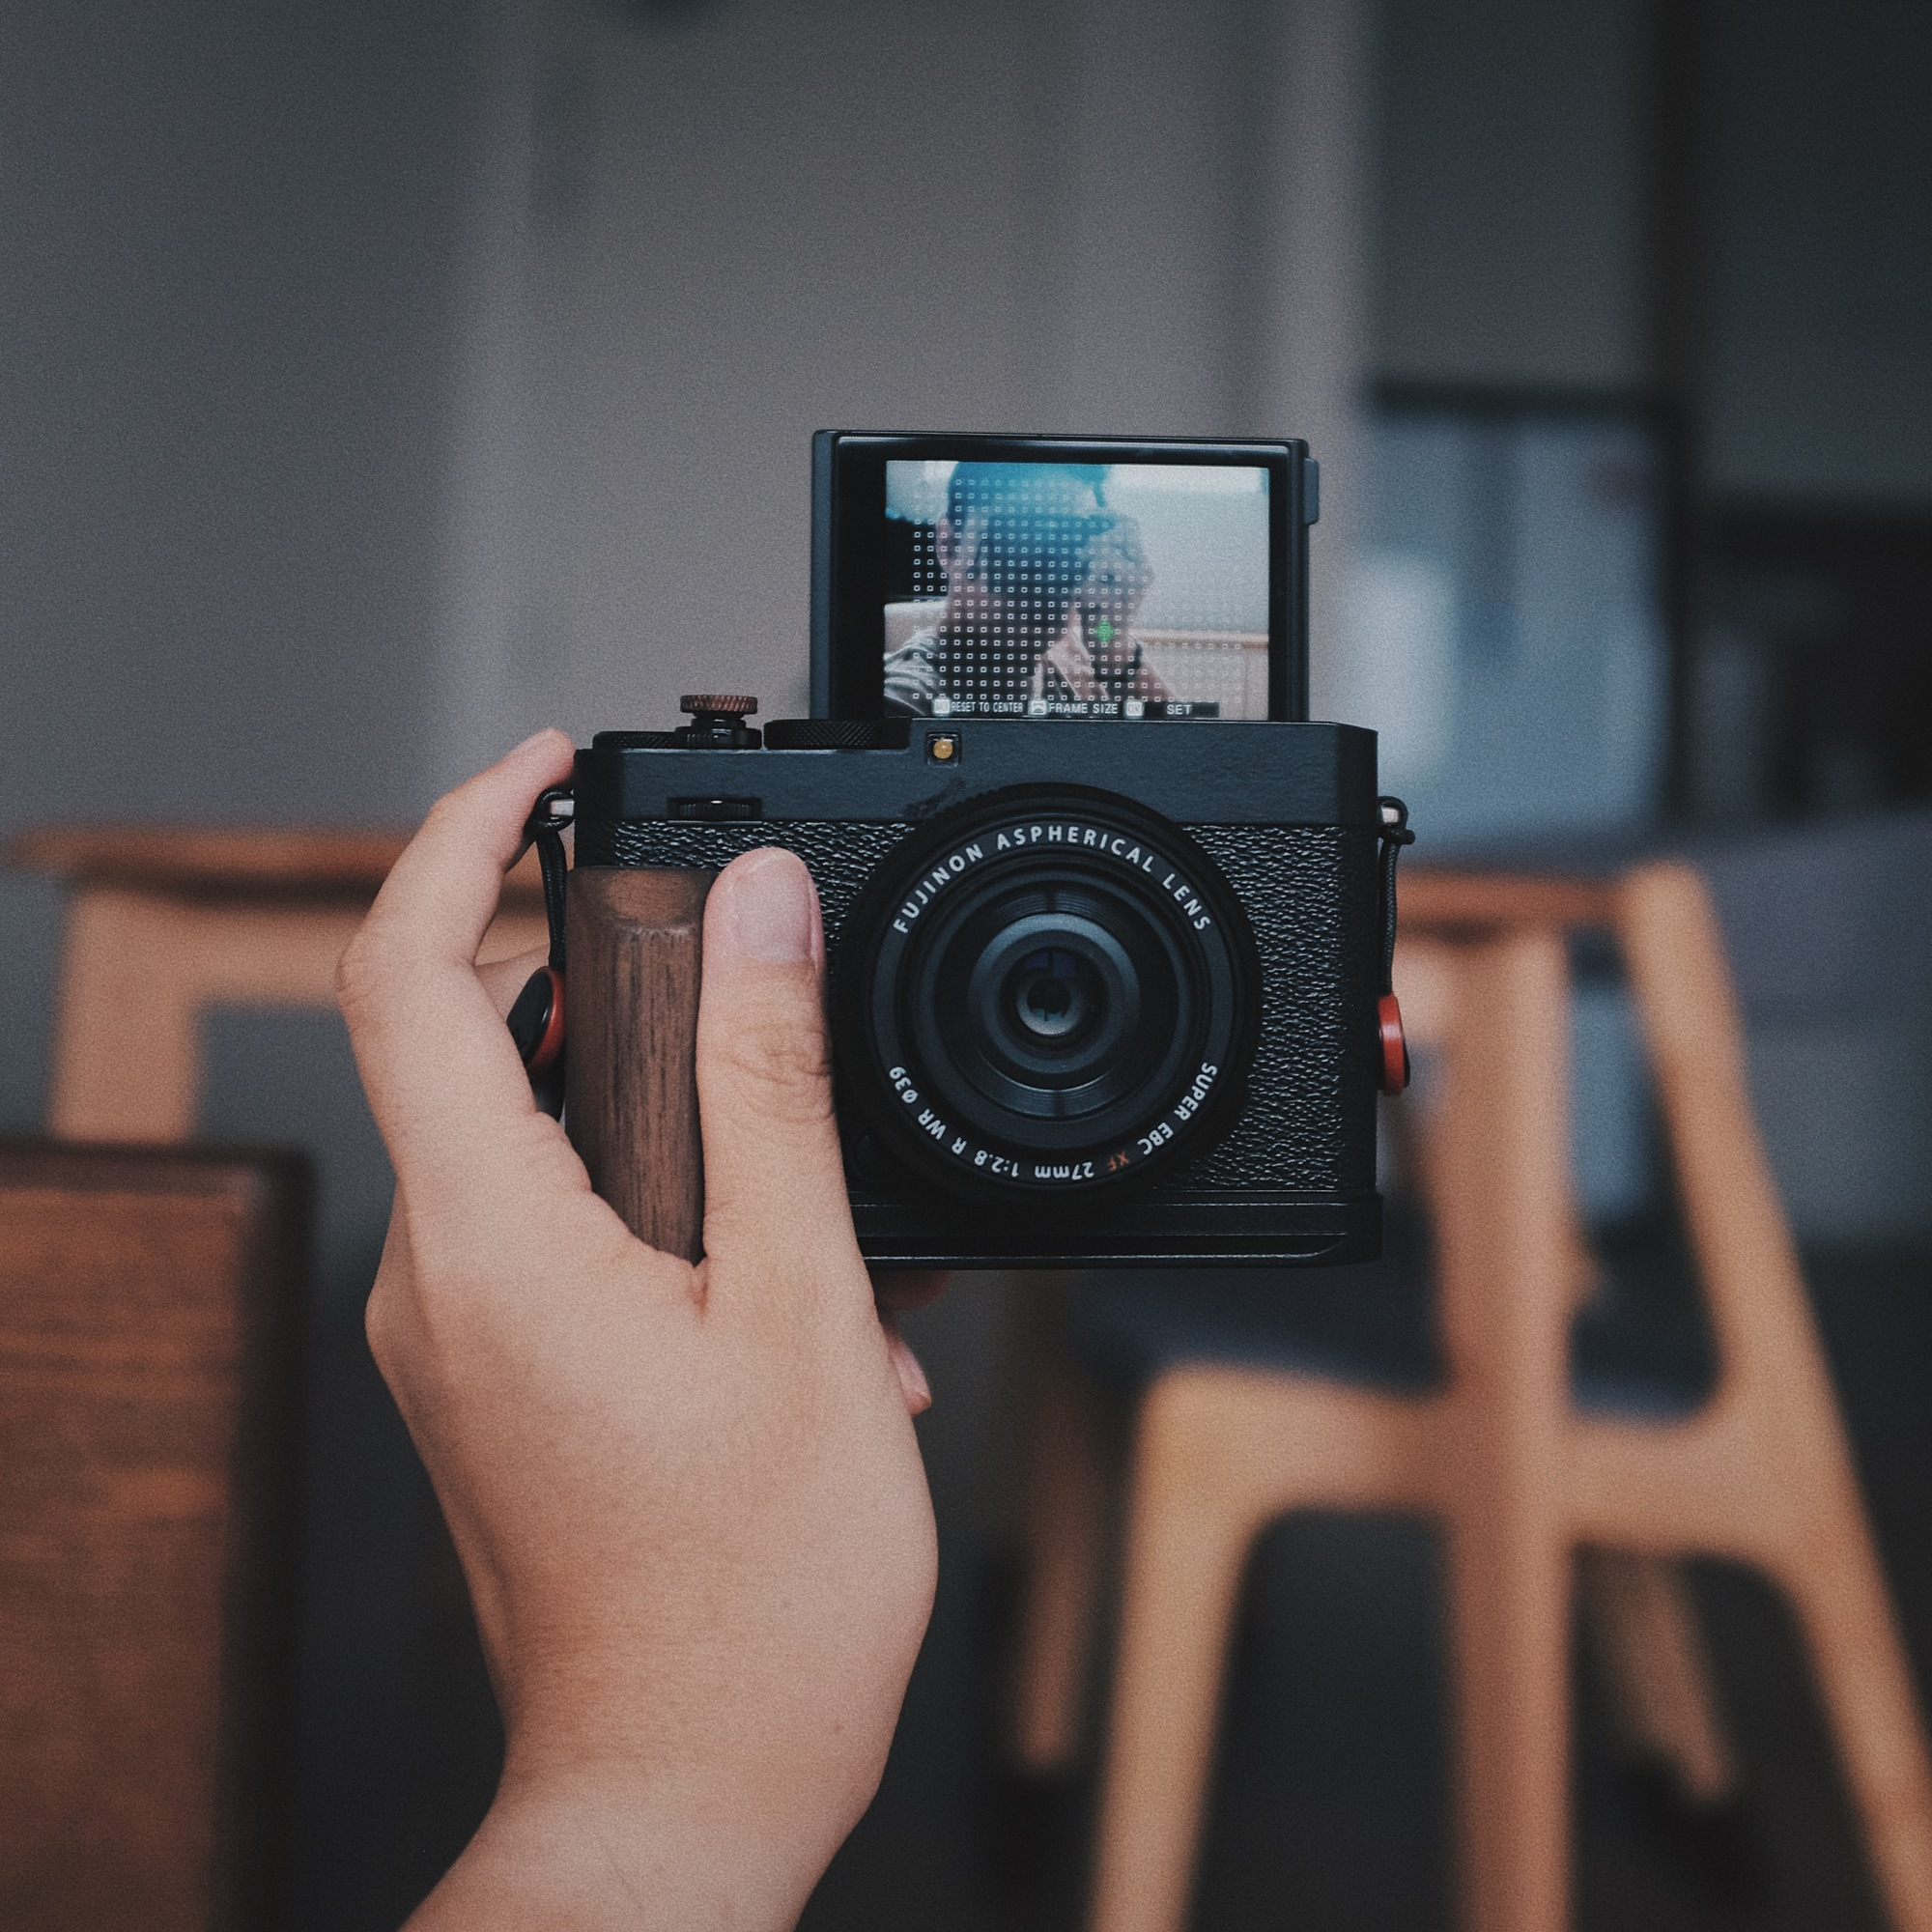
\includegraphics[width=\linewidth]{\envfinaldir/coverpic-prod.jpg}\par
            % \vskip 30pt
            \vfill

            \normalsize\rmfamily\scshape
            \copyright{} The Web Digest Project \hfill\large \envdatestr
        \end{center}
    \end{titlepage}
    % \restoregeometry
}
\newcommand{\simplehref}[1]{%
    \textcolor{blue!80!green}{\href{#1}{#1}}%
}
\renewcommand{\contentsname}{\center\Huge\sffamily\bfseries Contents\par\vskip 20pt}
\newcounter{ipartcounter}
\setcounter{ipartcounter}{0}
\newcommand{\ipart}[1]{
    % \vskip 20pt
    \clearpage
    \stepcounter{ipartcounter}
    \phantomsection
    \addcontentsline{toc}{chapter}{#1}
    % \begin{center}
    %     \Huge
    %     \sffamily\bfseries
    %     #1
    % \end{center}
    % \vskip 20pt plus 7pt
}
\newcounter{ichaptercounter}
\setcounter{ichaptercounter}{0}
\newcommand{\ichapter}[1]{
    % \vskip 20pt
    \clearpage
    \stepcounter{ichaptercounter}
    \phantomsection
    \addcontentsline{toc}{section}{\numberline{\arabic{ichaptercounter}}#1}
    \begin{center}
        \Huge
        \sffamily\bfseries
        #1
    \end{center}
    \vskip 20pt plus 7pt
}
\newcommand{\entrytitlefont}[1]{\subsection*{\raggedright\Large\sffamily\bfseries#1}}
\newcommand{\entryitemGeneric}[2]{
    % argv: title, url
    \parbox{\linewidth}{
        \entrytitlefont{#1}\par\vskip 5pt
        \footnotesize\ttfamily\mdseries
        \simplehref{#2}
    }\vskip 11pt plus 11pt minus 1pt
}
\newcommand{\entryitemGithub}[3]{
    % argv: title, url, desc
    \parbox{\linewidth}{
        \entrytitlefont{#1}\par\vskip 5pt
        \footnotesize\ttfamily\mdseries
        \simplehref{#2}\par\vskip 5pt
        \small\rmfamily\mdseries#3
    }\vskip 11pt plus 11pt minus 1pt
}
\newcommand{\entryitemAp}[3]{
    % argv: title, url, desc
    \parbox{\linewidth}{
        \entrytitlefont{#1}\par\vskip 5pt
        \footnotesize\ttfamily\mdseries
        \simplehref{#2}\par\vskip 5pt
        \small\rmfamily\mdseries#3
    }\vskip 11pt plus 11pt minus 1pt
}
\newcommand{\entryitemHackernews}[3]{
    % argv: title, hnurl, rawurl
    % \parbox{\linewidth}{
    %     \entrytitlefont{#1}\par\vskip 5pt
    %     \footnotesize\ttfamily\mdseries
    %     \simplehref{#3}\par
    %     \textcolor{black!50}{\href{#2}{#2}}
    % }\vskip 11pt plus 11pt minus 1pt
    \begin{minipage}{\linewidth}
            \entrytitlefont{#1}\par\vskip 5pt
            \footnotesize\ttfamily\mdseries
            \simplehref{#3}\par
            \textcolor{black!50}{\href{#2}{#2}}
    \end{minipage}\par\vskip 11pt plus 11pt minus 1pt
}







\begin{document}

\makeheader

\tableofcontents\clearpage




\ipart{Developers}
\ichapter{Hacker News}
\entryitemTwoLinks{Middle-aged man trading cards go viral in rural Japan town}{https://news.ycombinator.com/item?id=43615912}{https://www.tokyoweekender.com/entertainment/middle-aged-man-trading-cards-go-viral-in-japan/}

\entryitemTwoLinks{Agenda Behind the Facial Recognition Tech Used by ICE and the FBI Revealed}{https://news.ycombinator.com/item?id=43614592}{https://www.motherjones.com/politics/2025/04/clearview-ai-immigration-ice-fbi-surveillance-facial-recognition-hoan-ton-that-hal-lambert-trump/}

\entryitemTwoLinks{Show HN: Lux – A luxurious package manager for Lua}{https://news.ycombinator.com/item?id=43614285}{https://mrcjkb.dev/posts/2025-04-07-lux-announcement.html}

\entryitemTwoLinks{20 years of Git}{https://news.ycombinator.com/item?id=43613305}{https://blog.gitbutler.com/20-years-of-git/}

\entryitemTwoLinks{Show HN: Browser MCP – Automate your browser using Cursor, Claude, VS Code}{https://news.ycombinator.com/item?id=43613194}{https://browsermcp.io/}

\entryitemTwoLinks{LLMs understand nullability}{https://news.ycombinator.com/item?id=43612211}{https://dmodel.ai/nullability-gentle/}

\entryitemTwoLinks{Foreign visits into the U.S. fell off a cliff in March}{https://news.ycombinator.com/item?id=43610527}{https://www.axios.com/2025/04/04/foreign-visits-american-airports-travel-warnings}

\entryitemTwoLinks{Fewer Foreign Passengers Are Flying to the US}{https://news.ycombinator.com/item?id=43610246}{https://jasher.substack.com/p/how-fewer-foreign-passengers-flying}

\entryitemTwoLinks{The Dire Wolf Is Back}{https://news.ycombinator.com/item?id=43609661}{https://www.newyorker.com/magazine/2025/04/14/the-dire-wolf-is-back}

\entryitemTwoLinks{A startup doesn't need to be a unicorn}{https://news.ycombinator.com/item?id=43609242}{https://mattgiustwilliamson.substack.com/p/your-startup-doesnt-need-to-be-a}

\entryitemTwoLinks{Writing C for Curl}{https://news.ycombinator.com/item?id=43608551}{https://daniel.haxx.se/blog/2025/04/07/writing-c-for-curl/}

\entryitemTwoLinks{CDC's top laboratory on STDs is shut by Trump administration}{https://news.ycombinator.com/item?id=43607929}{https://www.statnews.com/2025/04/05/cdc-sexually-transmitted-diseases-laboratory-closed-by-trump-administration/}

\entryitemTwoLinks{Bill to block OpenAI's for-profit conversion gets mysteriously gutted}{https://news.ycombinator.com/item?id=43607502}{https://garymarcus.substack.com/p/breaking-bill-that-would-have-blocked}

\entryitemTwoLinks{Circuit breaker triggered in Japan for stock futures trading}{https://news.ycombinator.com/item?id=43606713}{https://www.wsj.com/livecoverage/stock-market-trump-tariffs-trade-war-04-07-25/card/circuit-breaker-triggered-in-japan-for-stock-futures-trading-Q5iMfZyfPGBEslrIObgB}

\entryitemTwoLinks{Let's Ban Billboards}{https://news.ycombinator.com/item?id=43606371}{https://iambateman.com/articles/billboards}

\entryitemTwoLinks{After 'coding error' triggers firings, top NIH scientists called back to work}{https://news.ycombinator.com/item?id=43606315}{https://www.science.org/content/article/after-coding-error-triggers-firings-top-nih-scientists-called-back-work}

\entryitemTwoLinks{Glamorous Toolkit}{https://news.ycombinator.com/item?id=43606027}{https://gtoolkit.com//}

\entryitemTwoLinks{SciOp torrents: download, seed erased US Gov sites and datasets}{https://news.ycombinator.com/item?id=43605751}{https://sciop.net/uploads/}

\entryitemTwoLinks{Baby Steps into Genetic Programming}{https://news.ycombinator.com/item?id=43605731}{https://aerique.blogspot.com/2011/01/baby-steps-into-genetic-programming.html}

\entryitemTwoLinks{Data centers contain 90\% crap data}{https://news.ycombinator.com/item?id=43605695}{https://gerrymcgovern.com/data-centers-contain-90-crap-data/}\ichapter{Phoronix}
\entryitemGeneric{\hskip 0pt{}Rust-Written Redox OS Makes USB 3.x Improvements, Async NVMe Driver Support}{https://www.phoronix.com/news/Redox-OS-March-2025}

\entryitemGeneric{\hskip 0pt{}Mozilla Builders' LocalScore: An Interesting Local AI LLM Benchmark}{https://www.phoronix.com/news/LocalScore-AI-LLM-Benchmark}

\entryitemGeneric{\hskip 0pt{}Ubuntu 25.04 Boosting AMD EPYC 9005 Performance Even Higher: ~14\% Faster Than Ubuntu 24.04 LTS}{https://www.phoronix.com/review/amd-epyc-9005-ubuntu-2504}

\entryitemGeneric{\hskip 0pt{}DXVK 2.6.1 Released With More Bug Fixes \& Performance Optimizations}{https://www.phoronix.com/news/DXVK-2.6.1-Released}

\entryitemGeneric{\hskip 0pt{}Five Year Old Ubuntu Bug For NVIDIA Suspend/Resume Experience: Now Working On X11, Wayland Not Yet}{https://www.phoronix.com/news/NVIDIA-Ubuntu-2025-SnR}

\entryitemGeneric{\hskip 0pt{}FFmpeg Lands AES-NI Optimized Implementation For Big Speed-Up}{https://www.phoronix.com/news/FFmpeg-Faster-AES-NI}

\entryitemGeneric{\hskip 0pt{}Apple M1 / M2 / M3 Core Support Might Soon Be Merged For The GCC Compiler}{https://www.phoronix.com/news/Apple-Cores-GCC-Possibly-Soon}

\entryitemGeneric{\hskip 0pt{}Linux 6.14.1 Released With An Initial Set Of Fixes \& Hardware Quirks}{https://www.phoronix.com/news/Linux-6.14.1-Released}

\entryitemGeneric{\hskip 0pt{}Turbostat Utility Bumps 1024 CPU Core Limit To 8192 Cores After HPE Breaches It With 1152 Cores}{https://www.phoronix.com/news/Linux-6.15-Turbostat}\ichapter{Dribbble}
\entryitemGeneric{\hskip 0pt{}Educational Website on Space Pollution}{https://dribbble.com/shots/25860515-Educational-Website-on-Space-Pollution}

\entryitemGeneric{\hskip 0pt{}Going for Gold}{https://dribbble.com/shots/25861716-Going-for-Gold}

\entryitemGeneric{\hskip 0pt{}LA Kings Mexican Heritage Theme Night Art}{https://dribbble.com/shots/25862720-LA-Kings-Mexican-Heritage-Theme-Night-Art}

\entryitemGeneric{\hskip 0pt{}CRYSTAL PRT\_2 // Mobile Version}{https://dribbble.com/shots/25860264-CRYSTAL-PRT-2-Mobile-Version}

\entryitemGeneric{\hskip 0pt{}Atomiq Unused Logo Design}{https://dribbble.com/shots/25861903-Atomiq-Unused-Logo-Design}

\entryitemGeneric{\hskip 0pt{}Hexagon + Waves Abstract Logo Concept}{https://dribbble.com/shots/25860795-Hexagon-Waves-Abstract-Logo-Concept}

\entryitemGeneric{\hskip 0pt{}Downlink}{https://dribbble.com/shots/25860034-Downlink}

\entryitemGeneric{\hskip 0pt{}Ship Logo Design - Boat, Shield, Star, Waves}{https://dribbble.com/shots/25854151-Ship-Logo-Design-Boat-Shield-Star-Waves}

\entryitemGeneric{\hskip 0pt{}Investment fund bank hero shot}{https://dribbble.com/shots/25855871-Investment-fund-bank-hero-shot}

\entryitemGeneric{\hskip 0pt{}HR website}{https://dribbble.com/shots/25854264-HR-website}

\entryitemGeneric{\hskip 0pt{}GenesysGo®}{https://dribbble.com/shots/25857394-GenesysGo}

\entryitemGeneric{\hskip 0pt{}Jot Landing Page, Website Design, business web site}{https://dribbble.com/shots/25843658-Jot-Landing-Page-Website-Design-business-web-site}

\entryitemGeneric{\hskip 0pt{}Interactive Speed Slider}{https://dribbble.com/shots/25851176-Interactive-Speed-Slider}

\entryitemGeneric{\hskip 0pt{}Abstract}{https://dribbble.com/shots/25853030-Abstract}

\entryitemGeneric{\hskip 0pt{}Croc logo}{https://dribbble.com/shots/25852607-Croc-logo}

\entryitemGeneric{\hskip 0pt{}Logo Design Selection Q1 2025}{https://dribbble.com/shots/25852275-Logo-Design-Selection-Q1-2025}

\entryitemGeneric{\hskip 0pt{}Cloud Lightning}{https://dribbble.com/shots/25852815-Cloud-Lightning}

\entryitemGeneric{\hskip 0pt{}Helpfull - Logo Redesign}{https://dribbble.com/shots/25847828-Helpfull-Logo-Redesign}

\entryitemGeneric{\hskip 0pt{}ef monogram}{https://dribbble.com/shots/25847206-ef-monogram}

\entryitemGeneric{\hskip 0pt{}Outrigger Marketing Logo}{https://dribbble.com/shots/25848681-Outrigger-Marketing-Logo}

\entryitemGeneric{\hskip 0pt{}Wayflow Logo Design - Letter W, Waves, Flow}{https://dribbble.com/shots/25847473-Wayflow-Logo-Design-Letter-W-Waves-Flow}

\entryitemGeneric{\hskip 0pt{}Prana Symbol}{https://dribbble.com/shots/25847656-Prana-Symbol}

\entryitemGeneric{\hskip 0pt{}Letter G set}{https://dribbble.com/shots/25845864-Letter-G-set}

\entryitemGeneric{\hskip 0pt{}Vínföng Final Wordmark}{https://dribbble.com/shots/25848505-V-nf-ng-Final-Wordmark}


\ipart{Developers~~~~(zh-Hans)}
\ichapter{Solidot}
\entryitemGeneric{\hskip 0pt{}Z 世代重新发现了 Tumblr}{https://www.solidot.org/story?sid=80981}

\entryitemGeneric{\hskip 0pt{}三星扩大对华芯片出口}{https://www.solidot.org/story?sid=80980}

\entryitemGeneric{\hskip 0pt{}Midjourney 发布新模型 V7}{https://www.solidot.org/story?sid=80979}

\entryitemGeneric{\hskip 0pt{}Starliner 宇航员回顾其飞行经历}{https://www.solidot.org/story?sid=80978}

\entryitemGeneric{\hskip 0pt{}Meta 宣布最新模型 Llama 4 herd}{https://www.solidot.org/story?sid=80977}

\entryitemGeneric{\hskip 0pt{} 《星际公民(Star Citizen)》筹款突破八亿美元}{https://www.solidot.org/story?sid=80976}

\entryitemGeneric{\hskip 0pt{}一名微软雇员干扰了公司五十周年庆}{https://www.solidot.org/story?sid=80975}

\entryitemGeneric{\hskip 0pt{}特朗普再给予 TikTok 75 天宽限期}{https://www.solidot.org/story?sid=80974}

\entryitemGeneric{\hskip 0pt{}天文学家在附近发现将碰撞的双星系统}{https://www.solidot.org/story?sid=80973}\ichapter{V2EX}
\entryitemGeneric{\hskip 0pt{}[问与答] 如何中美开战了,一些托管在美国服务怎么办?}{https://www.v2ex.com/t/1123844}

\entryitemGeneric{\hskip 0pt{}[宽带症候群] 上海联通 fttr 自带卫星路由器怎么样。}{https://www.v2ex.com/t/1123843}

\entryitemGeneric{\hskip 0pt{}[Apple] 苹果官网可以用国补吗?}{https://www.v2ex.com/t/1123842}

\entryitemGeneric{\hskip 0pt{}[发音] 请问一下,有没有教你正确发音的 APP 呢?比如可以慢读的发音。}{https://www.v2ex.com/t/1123841}

\entryitemGeneric{\hskip 0pt{}[程序员] alist 删库了,有人知道啥情况吗?}{https://www.v2ex.com/t/1123838}

\entryitemGeneric{\hskip 0pt{}[Apple] 苹果 writing-tool 正式出来之前,自己做了一个代替品 GinkgoGo}{https://www.v2ex.com/t/1123837}

\entryitemGeneric{\hskip 0pt{}[Mac mini] 求购买了 Mac Mini M4 的各位大佬帮忙测试一下 FFmpeg 转码影片速度}{https://www.v2ex.com/t/1123836}

\entryitemGeneric{\hskip 0pt{}[路由器] 梅林 380,如何修改立即更新的地址}{https://www.v2ex.com/t/1123835}

\entryitemGeneric{\hskip 0pt{}[问与答] qwen 帮我写代码,输出了一些乱七八糟的东西。}{https://www.v2ex.com/t/1123831}

\entryitemGeneric{\hskip 0pt{}[问与答] 个人开发者开发小程序如何盈利呢}{https://www.v2ex.com/t/1123830}

\entryitemGeneric{\hskip 0pt{}[Mac mini] xnip 在 mac mini 上用不了}{https://www.v2ex.com/t/1123828}

\entryitemGeneric{\hskip 0pt{}[分享发现] Alist 疑似被删库}{https://www.v2ex.com/t/1123827}

\entryitemGeneric{\hskip 0pt{}[Python] 想问下大家平时是怎么用 Python -Matplotlib 库画图}{https://www.v2ex.com/t/1123826}

\entryitemGeneric{\hskip 0pt{}[职场话题] 重生之我在愚人节为职场四宗罪背黑锅}{https://www.v2ex.com/t/1123825}

\entryitemGeneric{\hskip 0pt{}[分享发现] 试用了 browser use 的插件版 (nano browser) AI 成精了}{https://www.v2ex.com/t/1123824}

\entryitemGeneric{\hskip 0pt{}[问与答] Cloudflare 验证出问题了?}{https://www.v2ex.com/t/1123822}

\entryitemGeneric{\hskip 0pt{}[生活] 清明假期,高速小行,收获 80 辆应急车道违章!}{https://www.v2ex.com/t/1123821}

\entryitemGeneric{\hskip 0pt{}[WordPress] 调研,现在用 WordPress 的还多吗?}{https://www.v2ex.com/t/1123820}

\entryitemGeneric{\hskip 0pt{}[生活] 闲聊下,最近有点焦虑啊}{https://www.v2ex.com/t/1123819}

\entryitemGeneric{\hskip 0pt{}[生活] 也发一个生活贴,牛蛙不在了,一声叹息}{https://www.v2ex.com/t/1123818}

\entryitemGeneric{\hskip 0pt{}[分享发现] 分享一款安卓上的 T9 搜索应用小工具}{https://www.v2ex.com/t/1123817}

\entryitemGeneric{\hskip 0pt{}[香港] 今天办理了汇丰,但是没有当场下卡,要邮寄到国内,激活是不是还要再来一次香港啊?}{https://www.v2ex.com/t/1123816}

\entryitemGeneric{\hskip 0pt{}[分享发现] 专业编写标书售前方案智能工具!一键生成百万字标书的神器,写 P 标基本无需改动内容}{https://www.v2ex.com/t/1123815}

\entryitemGeneric{\hskip 0pt{}[问与答] 谷歌广告 iframe 嵌入展示问题}{https://www.v2ex.com/t/1123814}

\entryitemGeneric{\hskip 0pt{}[投资] 今天大 A 有割肉的吗?聊聊你认为的后续走势}{https://www.v2ex.com/t/1123813}

\entryitemGeneric{\hskip 0pt{}[Android] OPPO Find X8s AI 获取其他 APP 完整内容的技术实现+版权问题?}{https://www.v2ex.com/t/1123812}

\entryitemGeneric{\hskip 0pt{}[小米] 对于小米汽车此次事件的一些思考}{https://www.v2ex.com/t/1123811}

\entryitemGeneric{\hskip 0pt{}[OpenWrt] 有没有支持 OpenWrt 的随身 Wi-Fi}{https://www.v2ex.com/t/1123810}

\entryitemGeneric{\hskip 0pt{}[分享发现] 个人认为比较有深度的中国社会分析视频 [转]}{https://www.v2ex.com/t/1123809}

\entryitemGeneric{\hskip 0pt{}[Vim] coc.nvim 近期的主要更新}{https://www.v2ex.com/t/1123808}

\entryitemGeneric{\hskip 0pt{}[问与答] ai 编程英语提问给的代码似乎更好吗?}{https://www.v2ex.com/t/1123807}

\entryitemGeneric{\hskip 0pt{}[奇思妙想] 感觉已经把所有 5 分以上的科幻片都看过至少一遍🤣}{https://www.v2ex.com/t/1123806}

\entryitemGeneric{\hskip 0pt{}[旅行] 甲亢哥中国行最近很火呀}{https://www.v2ex.com/t/1123805}

\entryitemGeneric{\hskip 0pt{}[NAS] 分享无线程限制的 1.37.0 版本 Aria2,已打包为静态版本和 Docker 版本}{https://www.v2ex.com/t/1123804}

\entryitemGeneric{\hskip 0pt{}[问与答] 好哥哥们救救我,面试 gap 问题}{https://www.v2ex.com/t/1123803}

\entryitemGeneric{\hskip 0pt{}[职场话题] 内推前司失败,说我不够拼搏???}{https://www.v2ex.com/t/1123802}

\entryitemGeneric{\hskip 0pt{}[程序员] cursor 使用中误点了 stop,该怎样才能继续?}{https://www.v2ex.com/t/1123801}

\entryitemGeneric{\hskip 0pt{}[分享发现] 初试小红书起号, 3 天涨粉 500+,不到一周被限流}{https://www.v2ex.com/t/1123800}

\entryitemGeneric{\hskip 0pt{}[程序员] Cursor 取消了 Codebase 这么好用的功能,真是令人费解}{https://www.v2ex.com/t/1123799}

\entryitemGeneric{\hskip 0pt{}[信息安全] 公司电脑根目录下有一些莫名的文件,是病毒还是系统组件?}{https://www.v2ex.com/t/1123798}

\entryitemGeneric{\hskip 0pt{}[问与答] deepseek api 的缓存命中能关吗,每次结果都一样!}{https://www.v2ex.com/t/1123797}

\entryitemGeneric{\hskip 0pt{}[程序员] 聊聊 AI 时代下的 AI 生成代码直接部署的实现}{https://www.v2ex.com/t/1123791}

\entryitemGeneric{\hskip 0pt{}[问与答] 求推荐你们去香港住过的自我感觉高性价比的酒店}{https://www.v2ex.com/t/1123790}

\entryitemGeneric{\hskip 0pt{}[问与答] 最近想入手一台小主机,求推荐}{https://www.v2ex.com/t/1123789}

\entryitemGeneric{\hskip 0pt{}[职场话题] 上班越来越像打杂,面试要求却越来越高}{https://www.v2ex.com/t/1123788}

\entryitemGeneric{\hskip 0pt{}[求职] 北京 8 年 Python 后端求机会}{https://www.v2ex.com/t/1123787}

\entryitemGeneric{\hskip 0pt{}[职场话题] 兄弟们, 30 了,不想再干 Java 了,有什么其它行业信息交流下吗?}{https://www.v2ex.com/t/1123786}

\entryitemGeneric{\hskip 0pt{}[iOS] iOS 的截图 bug 什么时候能修复}{https://www.v2ex.com/t/1123785}

\entryitemGeneric{\hskip 0pt{}[投资] 上上周满仓,上周开始后悔,这周更加满是后悔。。。}{https://www.v2ex.com/t/1123784}

\entryitemGeneric{\hskip 0pt{}[问与答] 网易爆米花刮削是真的好用,但是播放器却基本功能都残缺}{https://www.v2ex.com/t/1123782}


\ipart{Generic News}
\ichapter{AP News}
\entryitemWithDescription{\hskip 0pt{}Jay North, TV's mischievous Dennis the Menace, dies at 73}{https://apnews.com/article/42cb0be07d2f858a92576bc212964735}{}

\entryitemWithDescription{\hskip 0pt{}Alex Ovechkin breaks Wayne Gretzky's NHL career goals record by scoring his 895th}{https://apnews.com/article/6f42df7b99d4693cc3f5bd6aff009af4}{}

\entryitemWithDescription{\hskip 0pt{}John Lithgow wins best actor at the UK stage Olivier Awards for exploring Roald Dahl's dark side}{https://apnews.com/article/a27ea96685571e5908f744023601e845}{}

\entryitemWithDescription{\hskip 0pt{}`A Minecraft Movie' is smashing all box office projections}{https://apnews.com/article/3d2887d1d272a12767f0703eb77c629d}{}

\entryitemWithDescription{\hskip 0pt{}Pope makes surprise appearance at St. Peter's Square, 2 weeks after leaving hospital}{https://apnews.com/article/50973c32de3f6e2cc1fd9dc036968f70}{}

\entryitemWithDescription{\hskip 0pt{}Liverpool loses and Southampton's relegation is sealed before a deadlocked Manchester derby}{https://apnews.com/article/5c18de4d02718b424c3c08619e6e4d56}{}

\entryitemWithDescription{\hskip 0pt{}Malian singer Amadou Bagayoko dies at age 70}{https://apnews.com/article/3ed90c068ea63bd4d7718a67378e5cc2}{}

\entryitemWithDescription{\hskip 0pt{}Alex Ovechkin ties Wayne Gretzky's NHL record with his 894th goal}{https://apnews.com/article/fd01a2d7c9362b559ad161507b1655a1}{}

\entryitemWithDescription{\hskip 0pt{}`This has got to be a moment in America,' Cory Booker tells 1st town hall since record speech}{https://apnews.com/article/e5882bbbc0f27ab49aa55c9965956e72}{}

\entryitemWithDescription{\hskip 0pt{}Jaguar and Land Rover maker pauses shipments to US as it develops post-tariff plans}{https://apnews.com/article/ad5d4cfdca70975ab357e2cb5a8d698c}{}

\entryitemWithDescription{\hskip 0pt{}We got a behind-the-scenes look at Nintendo Switch 2. These are our thoughts}{https://apnews.com/article/63b0e49951ed09a9532ca55b4b35002e}{}

\entryitemWithDescription{\hskip 0pt{}Bye-bye, Helene, Milton and Beryl. Names from those nasty hurricanes are now retired}{https://apnews.com/article/57d1c2f83d8494d4a531479c638bd844}{}

\entryitemWithDescription{\hskip 0pt{}At 89, Fred Costello plays the organ on opening day in Rochester just like he has since 1977}{https://apnews.com/article/bf234264a40eb3d6fd1fd6103045379f}{}\ichapter{Reuters}
\entryitemWithDescription{\hskip 0pt{}Israeli military changes initial account of Gaza aid worker killings}{https://www.reuters.com/world/middle-east/israeli-military-changes-initial-account-gaza-aid-worker-killings-2025-04-06/}{The Israeli military has provided new details that changed its initial account of the killing of 15 emergency workers near the southern Gaza city of Rafah last month but said investigators were still examining the...}

\entryitemWithDescription{\hskip 0pt{}Indonesia will not retaliate against Trump tariff, official says}{https://www.reuters.com/world/indonesia-will-not-retaliate-against-trump-tariff-official-says-2025-04-06/}{Indonesia will not retaliate against U.S. President Donald Trump\textquotesingle s trade tariff on Southeast Asia\textquotesingle s largest economy, its senior economic minister said on Sunday in the government\textquotesingle s first...}

\entryitemWithDescription{\hskip 0pt{}Iran wants indirect talks with US, warns regional countries over strikes against it}{https://www.reuters.com/world/middle-east/iran-wants-indirect-talks-with-us-warns-regional-countries-over-strikes-against-2025-04-06/}{Although Iran has rejected U.S. President Donald Trump\textquotesingle s demand for direct talks, it wants to continue indirect negotiations through Oman, a longtime channel for messages between the rival states, said the official, who...}

\entryitemWithDescription{\hskip 0pt{}EU seeks unity in first strike back at Trump tariffs}{https://www.reuters.com/markets/eu-seeks-unity-first-strike-back-trump-tariffs-2025-04-06/}{The European Commission, which coordinates EU trade policy, will propose to members late on Monday a list of U.S. products to hit with extra duties in response to Trump\textquotesingle s steel and aluminium tariffs rather than the broader...}

\entryitemWithDescription{\hskip 0pt{}Blizzards blanket Moscow in snow after unusually mild winter}{https://www.reuters.com/world/europe/blizzards-blanket-moscow-snow-after-unusually-mild-winter-2025-04-06/}{Blizzards blanketed Moscow in snow on Sunday, covering Red Square in up to 10 cm (4 inches) of snow after an unusually mild winter in the Russian...}

\entryitemWithDescription{\hskip 0pt{}South Korea firefighting helicopter crashes, pilot dead, Yonhap reports}{https://www.reuters.com/world/asia-pacific/skorea-firefighting-helicopter-crashes-pilot-dead-yonhap-reports-2025-04-06/}{A firefighting helicopter in South Korea crashed on Sunday, killing its pilot, Yonhap News Agency...}

\entryitemWithDescription{\hskip 0pt{}US, Vietnamese businesses ask Trump to delay 46\% tariffs on Vietnam}{https://www.reuters.com/markets/us-vietnamese-businesses-ask-trump-delay-46-tariffs-vietnam-2025-04-06/}{U.S. and Vietnamese businesses have asked the Trump administration to delay its planned 46\% tariff on Vietnamese goods, saying the levy will hurt them and bilateral commercial...}

\entryitemWithDescription{\hskip 0pt{}South Korea assembly speaker proposes revising constitution to curb presidency}{https://www.reuters.com/world/asia-pacific/south-korea-assembly-speaker-proposes-revising-constitution-curb-presidency-2025-04-06/}{The speaker of South Korea\textquotesingle s parliament on Sunday proposed revising the constitution to curb presidential powers, citing public support for such a move after President Yoon Suk Yeol was ousted for declaring martial...}

\entryitemWithDescription{\hskip 0pt{}Russian missile strike kills one, injures three in Kyiv, Ukraine says}{https://www.reuters.com/world/europe/russia-launches-air-attack-kyiv-ukraines-military-says-2025-04-06/}{A Russian missile attack on Kyiv killed one man and injured three other people overnight, causing damage and fires in several districts in the biggest such attack on Ukraine for weeks, Ukrainian officials said on...}

\entryitemWithDescription{\hskip 0pt{}France, Algeria resume dialogue, but rocky path ahead}{https://www.reuters.com/world/france-algeria-resume-dialogue-rocky-path-ahead-2025-04-06/}{France and Algeria resume diplomatic dialogue on Sunday after months of bickering that have hurt Paris\textquotesingle{} economic interests in its former colony, seen mutual accusations of humiliation and stalled vital security...}

\entryitemWithDescription{\hskip 0pt{}Three injured in Russia's overnight attack on Mykolaiv, Ukraine says}{https://www.reuters.com/world/europe/three-injured-russias-overnight-attack-mykolaiv-ukraine-says-2025-04-06/}{Three women were injured and several fires broke out in a Russian air attack on the southern Ukrainian region of Mykolaiv late on Saturday, Ukraine\textquotesingle s officials...}

\entryitemWithDescription{\hskip 0pt{}Rains add to challenge for Myanmar quake relief, toll at 3,471}{https://www.reuters.com/sustainability/society-equity/rains-add-challenge-myanmar-quake-relief-toll-3471-2025-04-06/}{Rains fell on parts of earthquake-hit Myanmar over the weekend, which aid agencies said could complicate relief efforts and raise the risk of disease as the United Nations aid chief said more tents were needed to shelter those left...}

\entryitemWithDescription{\hskip 0pt{}Musk says he hopes for 'zero tariffs' between US and Europe}{https://www.reuters.com/world/europe/musk-says-he-hopes-zero-tariffs-between-us-europe-2025-04-05/}{U.S. tech-billionaire Elon Musk said on Saturday he hoped in future to see complete freedom of trade between the United States and Europe, speaking days after U.S. President Donald Trump announced tariffs on trading...}






\clearpage
\leavevmode\vfill
\footnotesize

Copyright \copyright{} 2023-2025 Neruthes and other contributors.

This document is published with CC BY-NC-ND 4.0 license.

The entries listed in this newsletter may be copyrighted by their respective creators.

This newsletter is generated by the Web Digest project.

The newsletters are also delivered via Telegram channel \CJKunderline{\href{https://t.me/webdigestchannel}{https://t.me/webdigestchannel}}.\\
RSS feed is available at \CJKunderline{\href{https://webdigest.pages.dev/rss.xml}{https://webdigest.pages.dev/rss.xml}}.

This newsletter is available in PDF at
\CJKunderline{\href{https://webdigest.pages.dev/}{https://webdigest.pages.dev/}}.

The source code being used to generate this newsletter is available at\\
\CJKunderline{\href{https://github.com/neruthes/webdigest}{https://github.com/neruthes/webdigest}}.

This newsletter is also available in
\CJKunderline{\href{http://webdigest.pages.dev/readhtml/\envyear/WebDigest-20250408.html}{HTML}} and
\CJKunderline{\href{https://github.com/neruthes/webdigest/blob/master/markdown/\envyear/WebDigest-20250408.md}{Markdown}}.


\coverpic{https://unsplash.com/photos/a-pink-hyacinth-blooms-in-a-green-garden-1oeJ8sN6G0E}{Alin Gavriliuc}


\end{document}
